\section{\textcolor[HTML]{D32F2F}{Designiterasjon 2: Axure}}
\label{design2}

Versjon to av designet ble laget i et program kalt Axure. Dette er et verktøy for prototyping, spesifisering og diagrammer. Her kan man planlegge en prototype, og lage en troverdig app. Det gjør det mulig for gruppen å teste den faktiske opplevelsen av bruk på testpersonene. Modellen blir interaktiv og responderer på klikk. Axure-modellen er med andre ord langt mer avansert enn den forrige prototypen som ble testet med Wizard-of-Oz.

\subsection{Designbeslutninger}
I denne versjonen ble tilbakemeldingene fra brukertesten tatt med. Det ble gjort flere endringer i designet, blant annet ble det lagt inn deleknapp for ønskelister slik at brukeren kan dele direkte på Facebook eller e-post. Boksene i appen ble også endret fra å ha bokser med runde hjørner til å ha firkantede hjørner. Dette ble gjort for å få et pent og gjennomgående design, ikke fordi det hadde noen funksjon ellers i appen. Det siste som ble endret var handlelisten. I dette stadiet er det nødvendig å ta valg innen font, farger og grafiske elementer. Det er veldig viktig med en kosistent design. Dersom alle skjermbildene i applikasjonen følger samme grafiske profil, vil brukeren lettere forstå heltheten, forbedre navigasjonen, samt få et helhetlig inntrykk.

\subsubsection{Navigasjon}
Å ha en meny i produktet ble fort avgjort som nødvendig for en god brukeropplevelse. En meny skal gjerne vise innholdet på en strukturert måte, slik at brukeren skal kunne velge mellom et sett med valg \cite[s.~166]{preece}. Menyer i interface er gjerne plassert i topp- eller bunnlinjen av skjermen, eller langs venstre side. Det er mange måter å gjøre dette på, og eksempler er lister, drop-down, pop-up, kontekstuelle, ekspanderende og scrolling. Gruppen valgte å gå for en enkel meny, siden det er få sider i designet og målet var at appen skulle være enklest mulig. Ved å bruke denne menyen blir det enklere for brukeren å navigere seg mellom de forskjellige skjermbildene. 

\subsubsection{Farger}
Farger er også viktig for å få en ideell brukeropplevelse. Farger i seg selv signaliserer mye til brukeren, men også valg av farger å komponere er avgjørende. Å lese en grønn tekst på rød bakgrunn er slitsomt for øynene, og det samme er turkis på grå bakgrunn\cite{esthetics}. Det optimale er svart på hvitt for god lesbarhet, men det velges ofte farger for å sprite opp designet. Da er det vanlig å lage en fargepalett, hvor de samme fargene går gjennom i hele designet. Siden Sirkus shopping har en rød profil, valgte gruppen å bruke denne rødfargen som primærfarge. Videre utformet gruppen en fargepalett på \textcolor[HTML]{0000FF}{\underline{www.materialpalette.com}}, som vist i Figur \ref{fig:fargepalett}.

\begin{figure}[H]
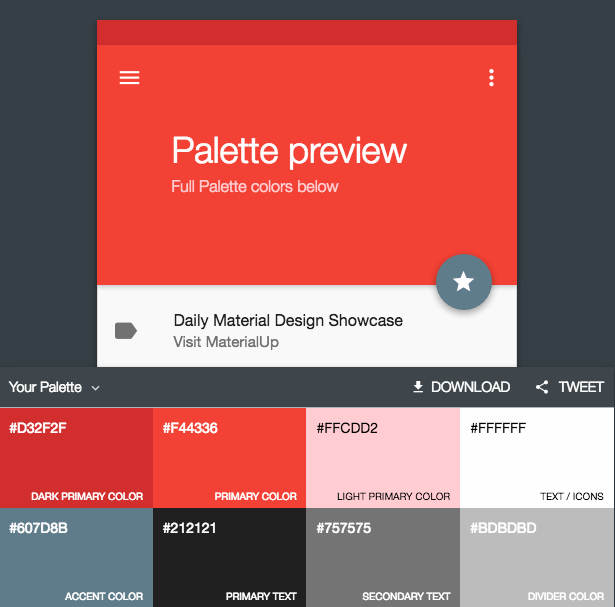
\includegraphics[scale=0.65]{images/colors.png}
\centering %centering the image
\caption{Applikasjonens fargepalett}
\label{fig:fargepalett}
\end{figure}

\subsubsection{Fonter}
Gruppen valgte å bruke Raleway som er en estetisk ren og lettleselig font. Det er viktig å ha en kontinuitet på fontstørrelse, og at hver størrelse har en mening. Det vil si å ha en fast stor størrelse på overskrifter, en mindre font på tekst for knapper, og en mindre font for infotekst. Med tanke på at applikasjonen skal benyttes av voksne mennesker, er det viktig å ha stor nok font for bra lesbarhet.

\subsubsection{Skjermbilder}
I Figur \ref{fig:interaksjon1} og Figur \ref{fig:interaksjon2} er det vist et diagram for å vise hvordan de forskjellige skjermbildene samhandler med hverandre. Figur \ref{fig:interaksjon1} viser hvordan du går fra login-skjerm til hovedmenyen. Herfra har du tre valg, der du kan enten opprette en ny ønskeliste, få en oversikt over ønskelistene dine, eller gå direkte til handlekurv. 

\begin{figure}[H]
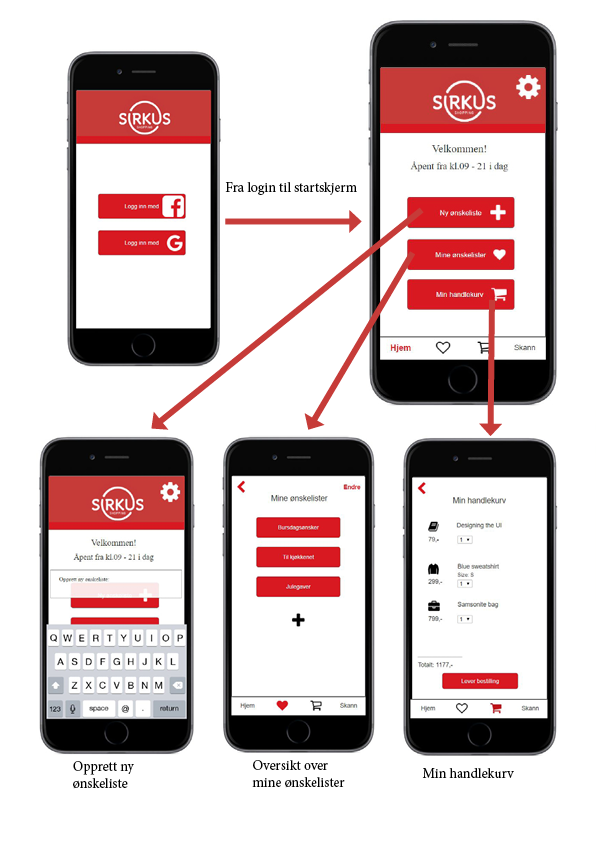
\includegraphics[scale=0.70]{images/axurebilder/axure-interaksjon.png}
\centering %centering the image
\caption{Interaksjon del 1}
\label{fig:interaksjon1}
\end{figure}

\noindent Figur \ref{fig:interaksjon2} viser hvordan brukeren kan trykke seg inn på et ønsket produkt fra handlekurven og deretter endre f.eks. størrelse. Dersom brukeren trykker på "Lever bestilling" blir hun dirigert til en ny skjerm som gir mulighet til å velge betalingsløsning. Herfra velger hun enten Vipps eller tradisjonell betaling i kasse. Etter å ha valgt her får brukeren et nytt skjermbilde som viser hvor lenge det er til hun kan hente varene sine. Det siste eksemplet viser hvordan man kan dele en ønskeliste via forskjellige sosiale plattformer.

\begin{figure}[H]
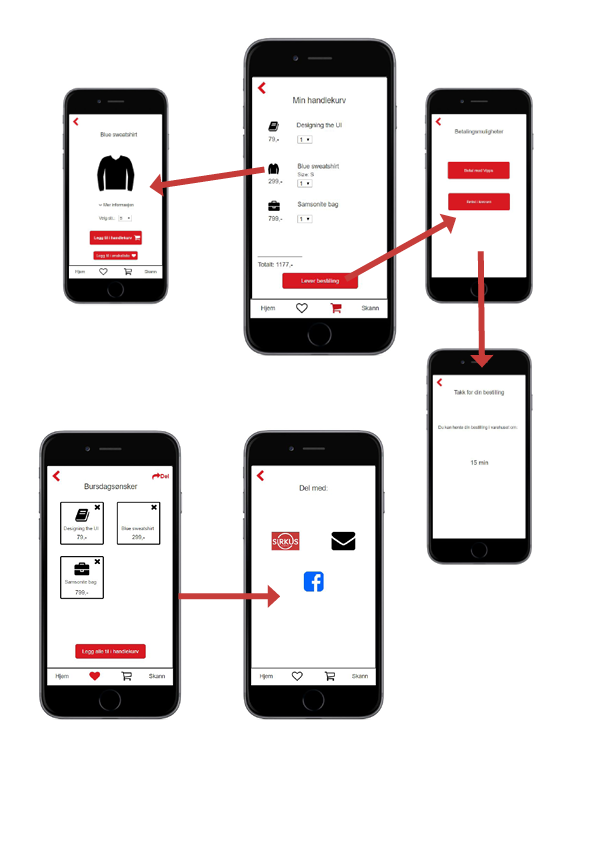
\includegraphics[scale=0.75]{images/axurebilder/interaksjon2}
\centering %centering the image
\caption{Interaksjon del 2}
\label{fig:interaksjon2}
\end{figure}

%flytdiagram

\subsection{Brukertest}
Da det skulle brukertestes gang nummer to, var det blitt laget en prototype med Axure. Denne prototypen lignet mye på det gruppen så for seg som det ferdige produktet, og denne brukertesten ble da av typen high-fidelity. Det vil si at den ligner mye på det ferdige produktet, og har flere funksjonaliteter enn en low-fidelity-prototype \cite[s.~391]{preece}. Å teste med high-fidelity har mange fordeler, siden det gir brukeren en nær opplevelse av hvordan det ferdige produktet vil se ut, men har også store kostnader. Det krever langt mer tid å utvikle en Axure-prototype enn en prototype i papir, slik gruppen brukte i Wizard-of-Oz-testen.

\subsubsection{Testprosedyre}
Den første brukertesten av Axure-prototypen ble gjort på lab hvor det ble brukt eyetracking. Dette er et kamera som er festet på undersiden av skjermen som detekterer hvor øynene ser. Før testen starter kalibrerer man programmet mot øynene, slik at man er sikker på at punktene brukeren ser på blir registrert. Deretter setter man kameraet på opptak, og vil da kunne se hvor brukeren ser til enhver tid, samt hvordan øynene forflytter seg over skjermen.
%les på forelesningsslide om eyetracking
\\\\\
Testspørsmålene som ble brukt under brukertesten var relativt like de som ble stilt i den forrige brukertesten. Dette ble gjort med hensikt, fordi det da er lettere å sammenligne resultatene. Noen endringer måtte likevel gjøres, siden appen hadde fått noen endrede funksjoner. Testspørsmålene er listet under.

\begin{enumerate}
    \item Logg inn med valgfritt innloggingsverktøy
    \item Du skal lage en oversikt over dine bursdagsønsker. Lista skal hete “bursdagsønsker”.
    \item Legg til en genser i listen over bursdagsønsker.
    \item Naviger deg tilbake til oversikten over mine ønskelister.
    \item Du er på oversikten over dine ønskelister. Naviger deg tilbake til startsiden.
    \item Genseren du har lagt i ønskelisten er i feil størrelse. Bytt størrelse.
    \item Del listen “Bursdagsønsker” med en venn. Velg selv delingsplattform.
    \item Slett ønskelisten “Julegaver”
    \item Gjennomfør et kjøp av denne genseren.
\end{enumerate}

\subsubsection{Resultat}
Den første oppgaven som ble gitt var å logge inn med et valgfritt innloggingsverktøy. Her valgte testpersonen å logge inn med Facebook, med en kommentar om at hun egentlig var litt skeptisk til å logge inn via dette. Ellers ble oppgaven løst uten problem. 
I oppgave to ble testpersonen bedt om å lage en oversikt over sine bursdagsønsker, og listen skulle hete “bursdagsønsker”. Brukeren trykket på ikonet for ny ønskeliste, skrev inn navn på listen og trykket “return” på tastaturet. Oppgaven ble løst vellykket.
\\\\
Neste oppgave var å legge til en genser i listen over bursdagsønsker. Her måtte brukeren tenke seg om før hun fant riktig løsning. Hun vurderte å trykke “legg til handlekurv” men konkluderte med at det ikke var det hun skulle gjøre. Hun trykket seg heller tilbake, og lette etter hvor det skulle gjøres. Siden det ikke ble gitt god nok informasjon i forkant av testen måtte testlederen bryte inn og minne om at produkter kan legges til ved å scanne varen. Da denne informasjonen ble påpekt hadde brukeren ingen problemer med å legge til varen i ønskelisten.
\\\\
Oppgaven var deretter å navigere seg tilbake til oversikten over ønskelister. Dette ble løst uten problem. Herfra fikk testpersonen i oppgave å navigere seg til startsiden. Hun nevner at hun både kan trykke på pil tilbake, og på huset nede i hjørnet for å komme seg tilbake. Hun velger å trykke på pilen. Oppgaven er løst.
\\\\
Neste oppgave testpersonen ble gitt var å endre størrelsen på genseren hun la til i ønskelisten. Brukeren lurer på hvilken størrelse hun skal endre til, men bestemmer seg for å bytte fra XS til M. Oppgaven er løst. Brukeren blir så bedt om å dele ønskelisten med en venn på en egenvalgt delingsplattform. Brukeren trykker på pilen i høyre hjørne og deler via Facebook. Hun får ingen respons på valget sitt, men blir fortalt at hun nå har delt listen. Deretter får hun oppgave i å slette ønskelisten kalt “Julegaver”. Brukeren går tilbake til oversikten over lister, og finner julegavelisten. Hun trykker på endre og sletter listen. Oppgaven er utført. Til slutt blir testpersonen bedt om å gjennomføre et kjøp av genseren. Hun legger genseren i handlekurven, leverer bestilling, betaler med Vipps og får beskjed om at varen kan hentes om 15 minutter.
\\\\
Etter testen tok testleder en prat med testpersonen om opplevelsen. Hun sa at noen ganger visste hun ikke hva hun skulle gjøre, men det gikk stort sett greit. Briefingen i forkant av testen ble ikke gjort godt nok, så testpersonen fikk ikke med seg det faktum at hun oppholdt seg på senteret. Ut over det mente hun at det nesten var umulig å gjøre feil i appen, siden det stort sett var to valg å velge mellom hele veien. Testlederen spurte om hva testpersonen tenkte om bruk av symboler som hjerte og handlevogn. Brukeren tok ikke i bruk menylinjen, med argument om at de var like på listene og i menyen. Hun kunne brukt de, men savnet tekst under ikonene i menyen. Hun skjønte at hjerte betydde favoritt, siden hjerte eller stjerne ofte symboliserer dette, men tok dem likevel ikke i bruk. Hadde hun brukt appen flere ganger hadde hun nok brukt ikonene, i følge henne selv. Konklusjonen fra testpersonen var at appen var enkel og ikke hadde unødvendige funksjoner. En siste kommentar var at det kanskje var unødvendig med ønskelisteikoner på forsiden.

\subsubsection{Analyse}
Gruppen valgte å bruke punkter og ikke ''heatmap'' for eyetrackingen, da skjermen er ganske liten og man mest sannsynlig kom til å se på midten av skjermen mye mer enn resten av skjermen. Med punkter får man se når og hvor man flytter blikket hele tiden.
\\\\
Siden det er ganske få elementer per skjermbilde og det meste i appen er sentrert, søker testpersonen som oftest i et vertikalt mønster opp og ned. Man kan observere at testpersonen skanner fort over elementene og bruker lite tid på å se nøye etter. Dette er ikke et problem her siden de fleste ordene og elementene er små at testpersonen får de med seg uten å måtte lese de. 
\\\\
Figur \ref{fig:eyetrack1} viser et bilde som er tatt noen sekunder etter at testpersonen har åpnet appen og startet med første oppgave. Her kan man se at testpersonen starter øverst med å lese åpningstidene og se på logoen. Etterhvert skanner hun nedover hovedmenyen for å se hva hun skal gjøre for å løse første oppgave. Hun ser ikke på menylinjen i det hele tatt før hun trykker på \textit{Ny ønskeliste} og fortsetter oppgaven. Det er en observasjon som gjentar seg gjennom hele testen. Blikket går veldig sjeldent ned på menylinjen, som bekrefter det testpersonen uttalte om at menylinjen fikk lite fokus siden man kunne navigere seg ved bruk av hjemskjermen og tilbakeknapper. 

\begin{figure}[H]
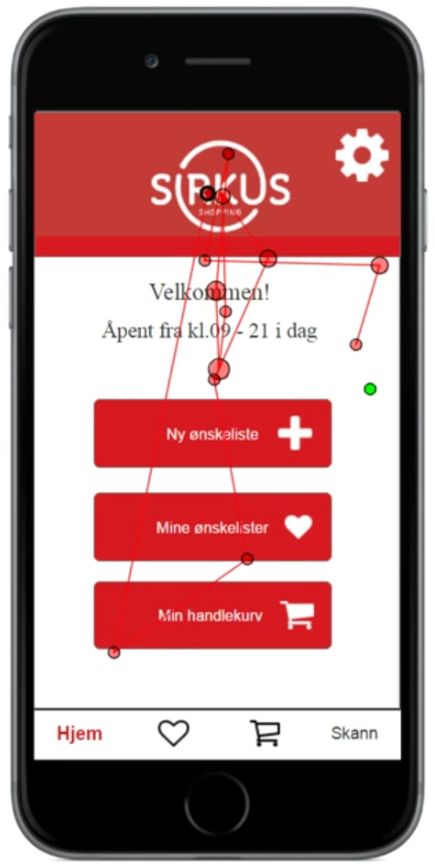
\includegraphics[scale=0.5]{images/eyetracking/eyetrack1.png}
\centering %centering the image
\caption{Eyetracking}
\label{fig:eyetrack1}
\end{figure}

%Videoen som ble tatt opp under testen
\noindent Det må nevnes at å brukerteste en applikasjon for mobiltelefon på en datamaskin ikke er helt ideelt. På en smarttelefon bruker man knapper på telefonen og touch-skjerm for å navigere i appen. På en datamaskin brukes en mus, så resultatene er ikke helt korrekt. 
